\documentclass{article}

\usepackage[colorlinks]{hyperref}
\usepackage{booktabs}
\usepackage{graphicx}
\usepackage[svgnames]{xcolor}
\usepackage{minted}
\usepackage{fancyvrb}

\usepackage[many]{tcolorbox}

% https://tex.stackexchange.com/questions/181082/how-to-reproduce-this-box-in-tcolorbox
\newtcbox{\srcbox}{
  enhanced,
  nobeforeafter,
  tcbox raise base,
  boxrule=0.4pt,
  top=0mm,
  bottom=0mm,
  right=0mm,
  left=4mm,
  arc=1pt,
  boxsep=2pt,
  before upper={\vphantom{dlg}},
  colframe=teal!75!white,
  coltext=teal!25!black,
  colback=teal!5!white,
  overlay={
    \begin{tcbclipinterior}
      \fill[teal!75!white] (frame.south west) rectangle node[text=white,font=\sffamily\bfseries\tiny,rotate=90] {SRC} ([xshift=4mm]frame.north west);
    \end{tcbclipinterior}
  }
}

\newtcolorbox{featurebox}[1]{colback=teal!5!white,colframe=teal!75!white,title={#1}}

%%% Local Variables:
%%% mode: latex
%%% TeX-master: "capernaum-architecture"
%%% End:

\usepackage[export]{adjustbox}

% GitHub links
\newcommand{\ghtag}{arch-doc}
\newcommand{\ghurlprefix}{https://github.com/quantum-bits/capernaum/blob/\ghtag}
\newcommand{\ghurl}[1]{\ghurlprefix/#1}
\newcommand{\ghsrc}[4]{
  \begin{tcolorbox}[
    skin=enhanced,
    after title={\hfill\textsf{source link}},
    colframe=blue!50!white,
    colback=blue!5!white,
    hyperurl=\ghurl{#3}/\#L#4,
    title={#1}]
    #2
  \end{tcolorbox}
}

\newcommand{\screensnap}[1]{\includegraphics[width=\textwidth,cframe=blue!50!white 1pt]{images/#1}}

% Names for things
\newcommand{\caper}{\textsc{Capernaum}}
\newcommand{\boil}{\textsc{BoilerPlate}}
\newcommand{\cli}{\textsc{Cli}}
\newcommand{\gh}{\textsc{GitHub}}
\newcommand{\rest}{\textsc{Rest}ful}
\newcommand{\unix}{\textsc{Unix}}
\newcommand{\linux}{\textsc{Linux}}

% Named URLs
\newcommand{\ansible}{\href{https://www.ansible.com/}{\textsc{Ansible}}}
\newcommand{\apollo}{\href{https://www.apollographql.com/}{\textsc{Apollo}}}
\newcommand{\axios}{\href{https://axios-http.com/}{\textsc{Axios}}}
\newcommand{\bg}{\href{https://www.biblegateway.com/}{Bible Gateway}}
\newcommand{\bull}{\href{https://www.npmjs.com/package/bull}{\textsc{Bull}}}
\newcommand{\cfse}{\href{https://www.taylor.edu/center-for-scripture-engagement/}{\textsc{C4SE}}}
\newcommand{\cls}{\href{https://www.taylor.edu/center-for-scripture-engagement/survey/}{\textsc{Cls}}}
\newcommand{\dotenv}{\href{https://www.npmjs.com/package/dotenv}{\textsc{dotenv}}}
\newcommand{\filepond}{\href{https://pqina.nl/filepond/}{\textsc{FilePond}}}
\newcommand{\git}{\href{https://git-scm.com/}{\textsc{Git}}}
\newcommand{\gql}{\href{https://graphql.org/}{\textsc{GraphQL}}}
\newcommand{\grafana}{\href{https://grafana.com/grafana/}{\textsc{Grafana}}}
\newcommand{\handlebars}{\href{https://handlebarsjs.com/}{\textsc{Handlebars}}}
\newcommand{\jwt}{\href{https://jwt.io/}{\textsc{Jwt}}}
\newcommand{\nest}{\href{https://nestjs.com/}{\textsc{Nest}}}
\newcommand{\nginx}{\href{https://www.nginx.com/}{\textsc{nginx}}}
\newcommand{\nodemailer}{\href{https://nodemailer.com/}{\textsc{Node\-mailer}}}
\newcommand{\node}{\href{https://nodejs.org/}{\textsc{Node}}}
\newcommand{\pg}{\href{https://www.postgresql.org/}{\textsc{PostgreSQL}}}
\newcommand{\pmtwo}{\href{https://pm2.keymetrics.io/}{\textsc{Pm2}}}
\newcommand{\prometheus}{\href{https://prometheus.io/}{\textsc{Prometheus}}}
\newcommand{\qual}{\href{https://www.qualtrics.com/}{\textsc{Qualtrics}}}
\newcommand{\redis}{\href{https://redis.io/}{\textsc{Redis}}}
\newcommand{\tiptap}{\href{https://tiptap.dev/}{\textsc{TipTap}}}
\newcommand{\ts}{\href{https://www.typescriptlang.org/}{\textsc{TypeScript}}}
\newcommand{\tu}{\href{https://www.taylor.edu/}{TU}}
\newcommand{\typeorm}{\href{https://typeorm.io/}{\textsc{TypeOrm}}}
\newcommand{\vega}{\href{https://vega.github.io/vega-lite/}{\textsc{Vega-Lite}}}
\newcommand{\vuetify}{\href{https://vuetifyjs.com/}{\textsc{Vuetify}}}
\newcommand{\vue}{\href{https://vuejs.org/}{\textsc{Vue}}}
\newcommand{\websocket}{\href{https://developer.mozilla.org/en-US/docs/Web/API/WebSockets_API}{\textsc{WebSocket}}}

%%% Local Variables:
%%% mode: latex
%%% TeX-master: "capernaum-architecture"
%%% End:

% LocalWords:  Capernaum Cli ful Ansible Axios se Cls GraphQL Grafana Jwt
% LocalWords:  Qualtrics TypeORM Vuetify


\title{Streamlined Application Development\\with \boil}
\author{Dr.\ Tom Nurkkala}

\begin{document}
\maketitle
\tableofcontents

\section{Introduction}
\label{sec:introduction}

Many components of a database-backed web application
depend critically
on the specifics of the database schema.
For example:
\begin{enumerate}
\item Object-Relational Mapper (ORM) model classes
\item Data transfer objects (DTO's)
\item Database service classes
\item RESTful API resources
\item GraphQL object types, input types, and resolvers
\item UI CRUD views that maintain database content
\end{enumerate}
Creating
and updating
such components manually
can be tedious, inconsistent, and error prone.
Different components
rely on different aspects
of the underlying database schema
and may employ different naming conventions and
coding practices.


\section{Architecture}
\label{sec:architecture}

\subsection{Overview}
\label{sec:overview}

\begin{figure}
  \centering
  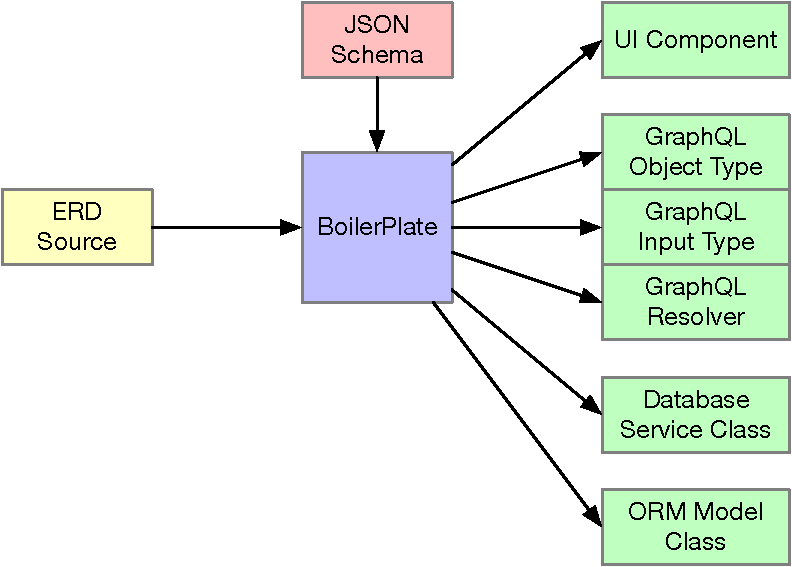
\includegraphics[width=\textwidth]{block-diagram}
  \caption{
    \boil{} block diagram.
    The \textsf{ERD Source} input file
    must conform to the \textsf{JSON Schema}.
    Based on command-line flags,
    \boil{} generates one or more output files.
  }
  \label{fig:block-diagram}
\end{figure}

\subsection{JSON Schema}
\label{sec:json-schema}

\boil{} defines
a \href{https://json-schema.org/}{JSON Schema}
for the ERD input file,
allowing it to validate the file at run time.
In addition,
IDE's like
\webstorm{}
can read the JSON schema
and provide syntax checking and code hinting
while editing the ERD input file.

\ghsrc{JSON Schema}{
  JSON Schema describing the format of the ERD input file
  accepted by \boil.
}{schemata/er-schema.json}{1}

\section{Usage}
\label{sec:usage}

This section considers the \hyperref[sec:command]{use of \boil},
including a \hyperref[sec:example]{simple example}.

\subsection{Command}
\label{sec:command}

Figure~\ref{fig:help} shows the help output
from the main \boil{} command, \texttt{boil}.

\begin{figure}[h]
  \centering
\begin{Verbatim}[frame=single,framerule=1pt,rulecolor=blue!50!white]
Usage: boil [options] <schema-file>

generate boilerplate from an ERD file

Options:
  -e --entity         generate entity
  -m --module         generate module
  -r --resolver       generate resolver
  -s --service        generate service
  -t --table          generate Vue table
  -c --create-update  generate Vue create-update
  -a --all            generate all
  -b --banner         show banner before each section
  -v --verbose        be verbose
  -h, --help          display help for command
\end{Verbatim}
  \caption{\boil{} help output}
  \label{fig:help}
\end{figure}

\subsection{Example}
\label{sec:example}

\begin{figure}[h]
  \centering
  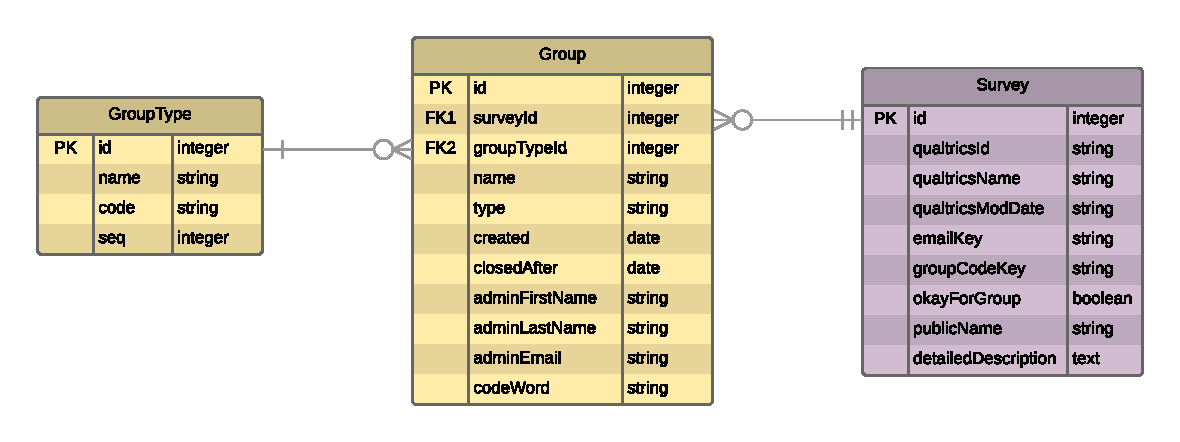
\includegraphics[width=\textwidth]{sample-erd}
  \caption{Entity-relationship diagram
    for the \texttt{Group}
    entity and entities related to it.
    The ERD source file for \texttt{Group}
    appears in Listing~\ref{listing:group-erd}.}
  \label{fig:erd}
\end{figure}

\begin{listing}
\begin{minted}[linenos,stepnumber=5,frame=single,fontsize=\small]{JSON}
{
  "entity": {
    "name": "Group",
    "pk": "id",
    "description": "Group of survey respondents",
    "attributes": [
      {
        "name": "name",
        "type": "string",
        "description": "Group name"
      },
      {
        "name": "closedAfter",
        "type": "string",
        "description": "Date when survey closes"
      },
      {
        "name": "adminEmail",
        "type": "string",
        "description": "Group administrator email address"
      },
      {
        "name": "codeWord",
        "type": "string",
        "description": "Survey code word used by group"
      }
    ]
  },
  "relationships": [
    {
      "name": "survey",
      "type": "manyToOne",
      "to": "Survey",
      "description": "Survey for this group"
    },
    {
      "name": "groupType",
      "type": "manyToOne",
      "to": "GroupType",
      "description": "Type for this group"
    }
  ]
}
\end{minted}
\caption{Sample ERD source file.
Several attributes have been removed
in order to fit the listing on a single page.}
\label{listing:group-erd}
\end{listing}

\end{document}

%%% Local Variables:
%%% mode: latex
%%% TeX-master: t
%%% End:

% LocalWords:  DTO's GraphQL
